\documentclass{CUP-JNL-DTM}%

%%%% Packages
\usepackage{graphicx}
\usepackage{multicol,multirow}
\usepackage{amsmath,amssymb,amsfonts}
\usepackage{mathrsfs}
\usepackage{amsthm}
\usepackage{rotating}
\usepackage{appendix}
\usepackage[numbers]{natbib}
\usepackage{ifpdf}
\usepackage[T1]{fontenc}
\usepackage{newtxtext}
\usepackage{newtxmath}
\usepackage{textcomp}
\usepackage{xcolor}
\usepackage{lipsum}
\usepackage[colorlinks,allcolors=blue]{hyperref}
\usepackage{jlcode} % for rendering Julia code
\usepackage{siunitx} 

%% formatting
\newtheorem{theorem}{Theorem}[section]
\newtheorem{lemma}[theorem]{Lemma}
\theoremstyle{definition}
\newtheorem{remark}[theorem]{Remark}
\newtheorem{example}[theorem]{Example}
\numberwithin{equation}{section}

% define how to display Julia
\newcommand{\Julia}{\texttt{Julia} }
\newcommand{\loss}{\mathcal{L}}
\newcommand{\net}{\mathcal{N}}
\newcommand{\Define}{\emph}

% Add line numbers
% \usepackage{lineno}
% \linenumbers

%\jname{Physics/Math}
\articletype{CAPSTONE PROJECT}
%\artid{20}
%\jyear{2022}
%\jvol{}
%\jissue{}
%\raggedbottom


\begin{document}

\begin{Frontmatter}

\title[Article Title]{Using Scientific Machine Learning to solve Partial Differential Equations}

\author{Miles Cochran-Branson}\orcid{0000-0002-8514-4315}
% \author[2]{Author Name2}\orcid{0000-0001-8823-831X}
% \author[2]{Author Name3}\orcid{0000-0002-0251-345}

\authormark{M. Cochran-Branson}

\address{\orgdiv{Department of Physics and Mathematics}, \orgname{Lawrence University}, \orgaddress{\city{Appleton}, \state{WI}}}%, \postcode{54911}, \country{USA}}}

%\address[2]{\orgdiv{Division}, \orgname{Organization}, \orgaddress{\city{City}, \postcode{Pincode}, \state{State},  \country{Country}}. \email{name2@email.com}}

\abstract{Machine learning and artificial intelligence have been used with great success in data science, mathematics, and physics as well as numerous other fields to solve complex or previously impossible problems. Computationally intensive problems in physics such as data analysis using a complex model and little data, or finding numerical solutions to differential equations have traditionally been solved with classical scientific computing techniques such as Taylor-series expansions or approximations using polynomials. Recent efforts have gone into replacing these techniques with neural networks and machine learning. Neural networks have the potential to fit any complex model or differential equation solution very accurately and can solve these problems quickly. In the following paper, we describe the basic principles of the growing field of Scientific Machine Learning (SciML).
(THIS WILL LIKELY CHANGE WITH MATURITY OF THE PROJECT): We will use the techniques we describe to solve the Einstein field equations to obtain the Schwarzschild metric using the package \texttt{NeuralPDE.jl} in the \Julia programming language. This example demonstrates the power a physics-informed neural network has in solving large, highly coupled systems of partial differential equations. }

\keywords{SciML, Scientific Computing, ML/AI, PINN, PDEs}

\end{Frontmatter}

\localtableofcontents

%% ---------------------------------------------------------------
%% SECTION: INTRODUCTION
%% ---------------------------------------------------------------

\section{Introduction}

An initiative laid out by the DOE in 2019 outlines the importance and potential of the ever growing field of Scientific Machine Learning (SciML) \cite{bakerWorkshopReportBasic2019}. In this report, they indicate the computational challenges SciML could potentially solve: lack of data in analysis, and solving differential equations. In the first case, in problems where data is either expensive or impossible to collect, implementations of machine learning become impossible. This can be overcome if we can incorporate physics knowledge of the system into the neural network. Such implementations make use of \emph{Physics-Informed Neural Networks} (PINN) \cite{karniadakisPhysicsinformedMachineLearning2021}. Additionally, PINN can solve differential equations by slight modification of the lack of data problem. We can even combine these two techniques by including data into solving differential equations to better fit a model or aid in solving the equation(s). A robust implementation of many of these techniques has been underway in the \Julia programming language. Packages that make use of machine learning are part of the \texttt{SciML.jl} universe which includes a basic syntax for code and basic functions in using SciML. Further information on the evolution of the SciML universe can be found in last year's SciML Con \cite{SciMLCon2022}. 

Because of the rapidly growing nature of the field of SciML, documentation on how the techniques are used and the new tools available are not easy to access. This paper seeks to fill in some of the gaps, describing succinctly how SciML can be used to solve differential equations. In particular, we put the newly-released package \texttt{NeuralPDE.jl} to the test to solve several complex differential equations and compare the computational solutions to known analytical solutions. In section two, we will outline the basics of what machine learning is. In sections three and four we will describe how to solve ODEs and PDEs with Physics-Informed Neural Networks (PINN). Finally, in section five we present a more complex problem: solving Einstein's field equations to obtain the Schwarzschild Metric using PINN. 

ADD HERE ONCE COMPLETED:
In the conclusions section I describe some future directions of this research and hopefully some suggestions? We shall see. Also findings?

%% ---------------------------------------------------------------
%% SECTION: MACHINE LEARNING
%% ---------------------------------------------------------------

\section{Machine Learning}

Machine learning and artificial intelligence are prominent features of our everyday life from personalized advertisements to facial recognition software. Machine learning is also a powerful analytical tool in scientific research, in particular with model development and validation. Below, I will describe how neural networks can be trained to make predictions and give some motivation for why neural networks are well suited for function approximation, in particular differential equation approximation. 

%% SUBSECTION: NEURAL NETWORKS %%

\subsection{Neural Networks}

A neural network is simply a function composed primarily of layers of matrix multiplication, but also of non-linear components---activation functions, and optionally addition of bias vectors within the function \cite{strangLinearAlgebraLearning2019, bishopPatternRecognitionMachine2006}. As input, a neural network can take a scalar, vector, matrix, or sometimes tensor with a user-specified size / dimension and gives as an output a vector or scalar. Thus, our network $\net$ takes the form

\begin{equation}
    \net : \mathbb{R}^{\Theta} \rightarrow \mathbb{R}^{\ell}
\end{equation}
where $\Theta$ is the user-defined input space, and $\ell$ is the number of desired output features. Networks have a fixed size defined by the number of \Define{hidden layers} and the number of \Define{nodes} each hidden layer has. 

Hidden layers are composed of nodes which cannot be directly accessed in the training process. A node within a layer describes a connection point between layers. Connections are achieved via multiplication by a weight stored in the network. Modification of these weights changes the way in which nodes are connected to each other and thus how inputs are interpreted by the network. At each node, the weight passed to the node is modified by a non-linear function called the \Define{activation function}. This allows us to describe a complex input space more accurately \cite{dubeyActivationFunctionsDeep2022a}. Some examples of activation functions include the sigmoid defined by 

\begin{equation}
    \sigma(w) = \frac{1}{1 + e^{-w}},
\end{equation}
the hyperbolic tangent $\tanh(w)$, and LSTM defined by $f(w) = \textrm{max}\{0,w\}$ where in each case $w$ are a vector of weights of the network at a node. Typically, the sigmoid is well suited for classification problems, while LSTM is best used in regression problems due to its simplicity. In examples presented later, we typically use a sigmoid activation function. 

An example of a simple neural network with one hidden layer is shown in Fig. \ref{fig:NNexample}. This network has one input dimension and, as shown in the graphic, we feed one data point $X$ with two features $x_1, x_2$ into the network. Parameters of the network are stored in the matrix $W_0$ such that when we do the multiplication $X W_0$ we get a vector of three values corresponding to the three nodes of the single hidden layer. The activation function is now applied to these values and optionally a bias vector can be added to these modified weights. We then multiply by the weights $W_1$ to get our output of a single value which is passed to one final activation function. In most cases, the activation in the final node is the identity function $f(x) = x$. Notice that we can have as many inputs, layers, nodes, and output nodes as we would like. The network described above is typically called a \Define{feed-forward} neural network as there are no cycles between nodes, no reference to nodes previously touched and each node from the previous layer is connected to each node of the subsequent layer. There are more complex neural networks such as recurrent neural networks which have these features, however, we will not use these in our work.

\begin{figure}
\centering
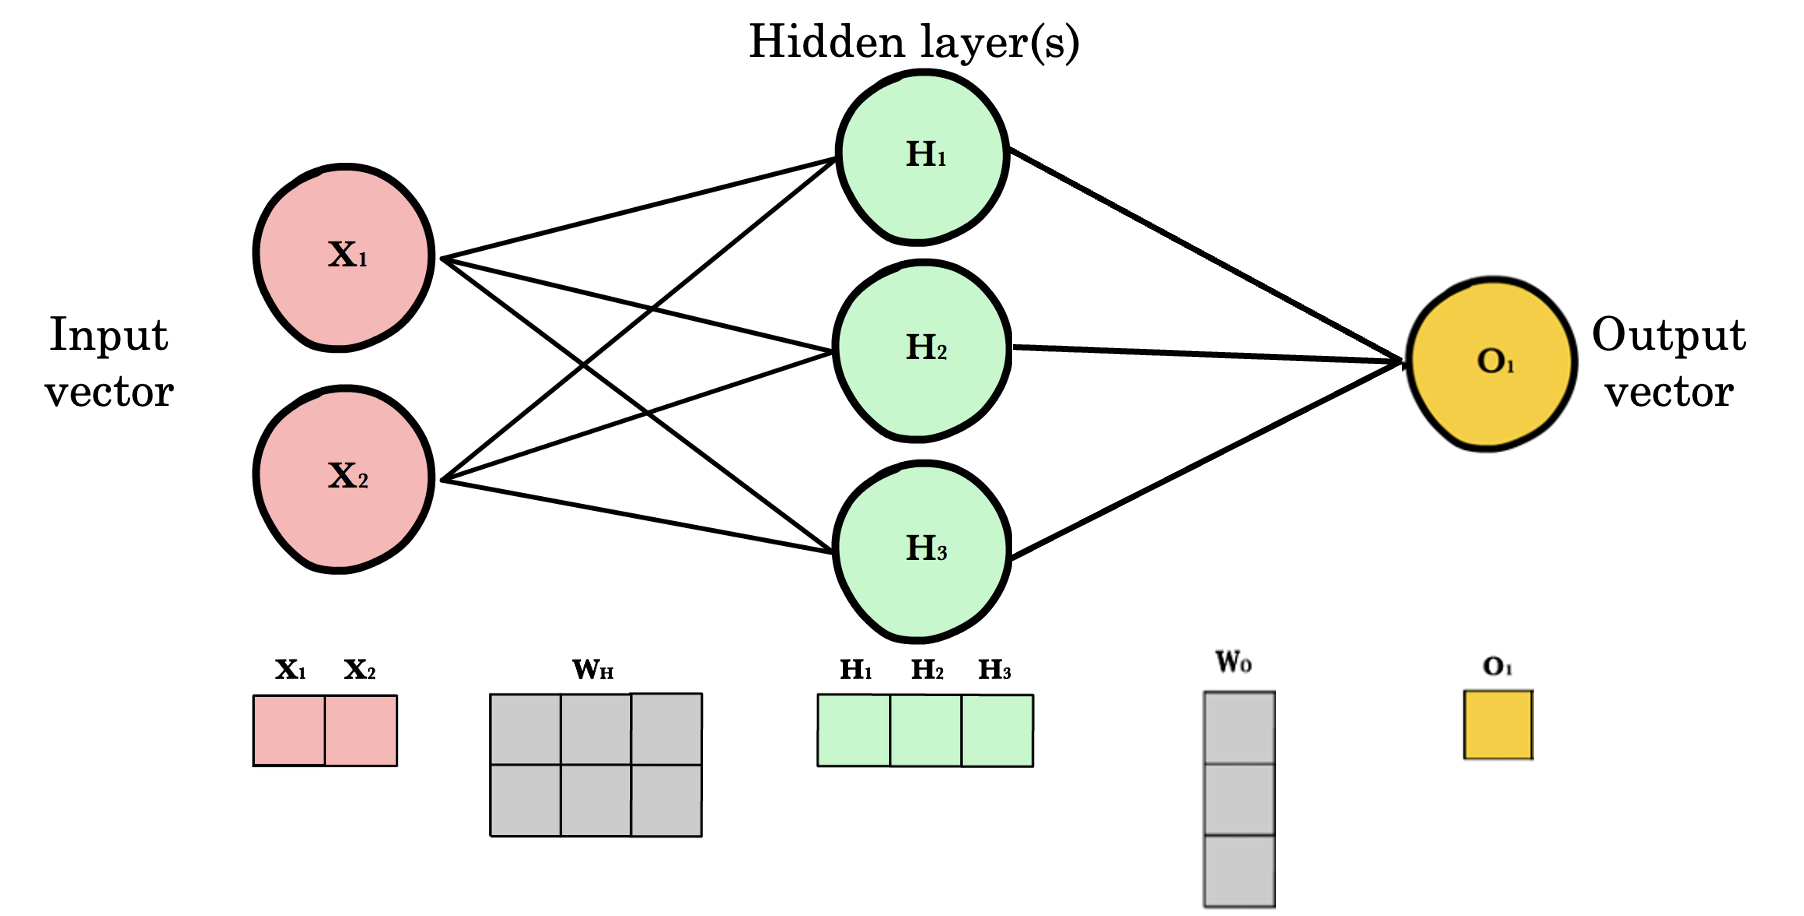
\includegraphics[width=0.7\linewidth]{figures/NN_example.png}
\caption{An example of a simple neural network with two inputs, one hidden layer with three nodes, and a single output. The network is defined by the weights connecting the layers which are represented as matrices. At each node, the weights are passed to a function called the activation function which scales the weights appropriately. In principle, the size of the network can change in every dimension}
\label{fig:NNexample}
\end{figure}


%% SUBSECTION: TRAINING NEURAL NETWORKS %% 

\subsection{Training Neural Networks}

Now that we have built some neural network, we would like to have it make some useful predictions. This involves picking a set of special weights through a process called \Define{training}. 

In order to train a neural network, we need a way in which to evaluate how well the network is doing given a specific task. This is achieved with a \emph{loss function}. The loss function takes an input of all of the parameters of the network that can change, $X$, and outputs a single number, thus, our loss function is of the form

\begin{equation}
    \loss : \mathbb{R}^{\textrm{size}(X)} \rightarrow \mathbb{R}. 
\end{equation}
Such a function is defined such that the smaller the output value, the better the network performs. Thus, training a neural network becomes an optimization problem where we want to minimize the function $\loss(X)$. Typically, the space $X$ is composed of the weights and biases of the network. 

For a very basic idea of how this works, imagine the space defined by $\loss$ as a surface with some collection of minima. We want to find a minimum, so we need to travel in the direction of one. Intuitively, we can take the gradient and then travel in the direction of the negative gradient to go ``downhill". More specifically, we travel in the $-\nabla \loss(X)$ direction taking discrete steps of size $\Delta x$. After each step we update the network parameters, re-evaluate the loss, compute $-\nabla \loss(X)$ and repeat. We continue in this way for as many steps as the user desires. This process is called gradient descent and the algorithm for finding the desired weights is called backpropogation \cite{chauvinBackpropagationTheoryArchitectures1995}. In most cases, it is not necessary to find the global minimum and may even be computationally disadvantageous as finding global minimum can lead to over-fitting \cite{choromanskaLossSurfacesMultilayer2015}. Because in some cases, learning can get stuck in a ``saddle point" or small local minimum, we often use stochastic methods which allow us to get out of such cases and continue learning to a minimum. This process is called stochastic gradient descent. In the following examples, we will use the ADAM optimizer which uses stochastic methods to find a minimum \cite{kingmaAdamMethodStochastic2017}. 

%% SUBSECTION: THE UAT %%

\subsection{The Universal Approximation Theorem}

A natural question when posing machine learning as a solution to PDEs is why this should work in the first place. The answer comes down to a famous theorem in machine learning: the Universal Approximation Theorem (UAT):

\begin{theorem}

Let $x \in \Omega$, let $u(x)$ be a regular function, and $\net(x,w)$ be a neural network with weights $w$. Then, we can find some arbitrarily small $\epsilon \in \Omega$ such that 

\begin{equation}
	||\net(x,w) - u(x)|| < \epsilon. 
\end{equation}

\end{theorem}

\noindent Proofs of this theorem are beyond the scope of this report, but are readily availible for several different contexts including for classical feed-forward networks \cite{hornikMultilayerFeedforwardNetworks1989, hornikApproximationCapabilitiesMultilayer1991}, finding probability distributions \cite{luUniversalApproximationTheorem2020}, and complex-valued neural networks \cite{voigtlaenderUniversalApproximationTheorem2020}. 

There is, however, one big caveat to this theorem: nothing about the problem tells us how big our network should be in order to fulfill the theorem. In some cases, the size of the network may be computationally infeasible to model. Nonetheless, it is this theorem which allows us to be able to have some hope that differential equations can be arbitrarily approximated by neural networks. 

In the rest of the paper, we take these theoretical concepts and apply them to the problem of solving differential equations, starting with ODEs and then moving to PDEs. 

\subsection{Differential Programming}

%% ---------------------------------------------------------------
%% SECTION: SOLVING ODES WITH PINN
%% ---------------------------------------------------------------

\section{Solving ODEs with Physics-Informed Neural Networks}

As an illustration of the application of PINN, consider an ordinary differential equation of the form 

\begin{equation}
	u' = f(u,t). 
\end{equation}
The UAT tells us that we should be able to achieve $N(w,t) \approx u(t)$ where $N(w,t)$ is a neural network with weights $w$. Consequently, our neural network must satisfy $N'(w,t) \approx f(N(w,t), t)$. To solve, we discretize the space $\Omega$ where $t \in \Omega$. Subsequently, we define the loss function by 

\begin{equation}
	\loss(w) = \sum_i \left( \frac{d\net(w, t_i)}{dt} - f(\net(w,t_i), t_i)\right)^2. 
\end{equation}
In order to find a unique solution, we apply the initial condition $u(0) = u_0$. We can simply add this to our loss function as 

\begin{equation}
	\loss(w) = (\net(w,0) - u_0)^2 + \sum_i \left( \frac{d\net(w,t_i)}{dt} - f(\net(w,t_i), t_i),\right)^2
\end{equation}
or we can parametrize the function to learn on, encoding the initial condition in our neural network solution by defining the function 

\begin{equation}
	g(w,t) = u_0 - t\net(w,t).
\end{equation}
This ensures that the initial condition is satisfied and allows us to write down a simpler version of the loss function:

\begin{equation}
	\loss(w) = \sum_i \left(\frac{dg(w,t_i)}{dt} - f(g(w,t_i), t_i)\right)^2. 
\end{equation}

Now that we have defined our problem, we can use standard minimization techniques to find a solution. For more information and further examples see \cite{rackauckasSciMLSciMLBookParallel}. 

\subsection{Example ODE problem solved with a PINN}
	
Consider the equation

\begin{equation}
	u' = e^t \cos t
\end{equation}
with the initial condition $u(0) = 0.1$. Notice that we can find the solution to this equation via integration, i.e., the solution is given by

\begin{equation}
	u(t) = \int e^t \cos t \, dt. 
\end{equation}
Applying integration by parts twice, we find the solution

\begin{equation}
	u(t) = \frac{1}{2}e^t(\sin t + \cos t) + C
\end{equation}
where $C = -0.4$ via use of the initial condition. 

Let's now solve using the techniques defined above using \Julia and the machine learning package \texttt{Flux.jl}. We begin by defining a neural network with two hidden layers one of 64 nodes the other with 32 nodes using the $\tanh$ activation function and a linear output: 

\begin{jllisting}
using Flux
NNODE = Chain(x -> [x], # Take in a scalar and transform it into an array
           Dense(1,64, tanh),
           Dense(64, 32, tanh),
           Dense(32,1),
           first) # Take first value, i.e. return a scalar
\end{jllisting}
We then parametrize the solution and define the loss function in which the differentiation is computed via discretization:

\begin{jllisting}
g(t) = t*NNODE(t) + 0.1

using Statistics
ϵ = sqrt(eps(Float32))
loss() = mean(abs2(((g(t+ϵ)-g(t))/ϵ) - (exp(t) * cos(t))) for t in 0:1f-2:5f0)
\end{jllisting}
Notice that we use machine $\epsilon$ here to discretize our integral as this is the smallest possible discretization before floating point error disrupts the solution. We will use gradient descent to solve with a learning rate of $10^{-4}$ over $10^4$ epochs. Because there is no data we are providing to train on, we feed the network empty data. Instead, all of the learning information comes from the loss function defined above. This is accomplished with the following code:

\begin{jllisting}
epochs = 10_000
learning_rate = 1e-4

opt = Flux.Descent(learning_rate) # use gradient Descent
data = Iterators.repeated((), epochs) # no data here : repeat empty data
iter = 0
loss_history = []
cb = function () #callback function to observe training
  global iter += 1
  push!(loss_history, loss())
  if iter % 500 == 0
    display(loss())
  end
end
display(loss())
Flux.train!(loss, Flux.params(NNODE), data, opt; cb=cb)
\end{jllisting}
We can then see how our network does in comparison to the true solution as shown in the below plot:

\begin{center}
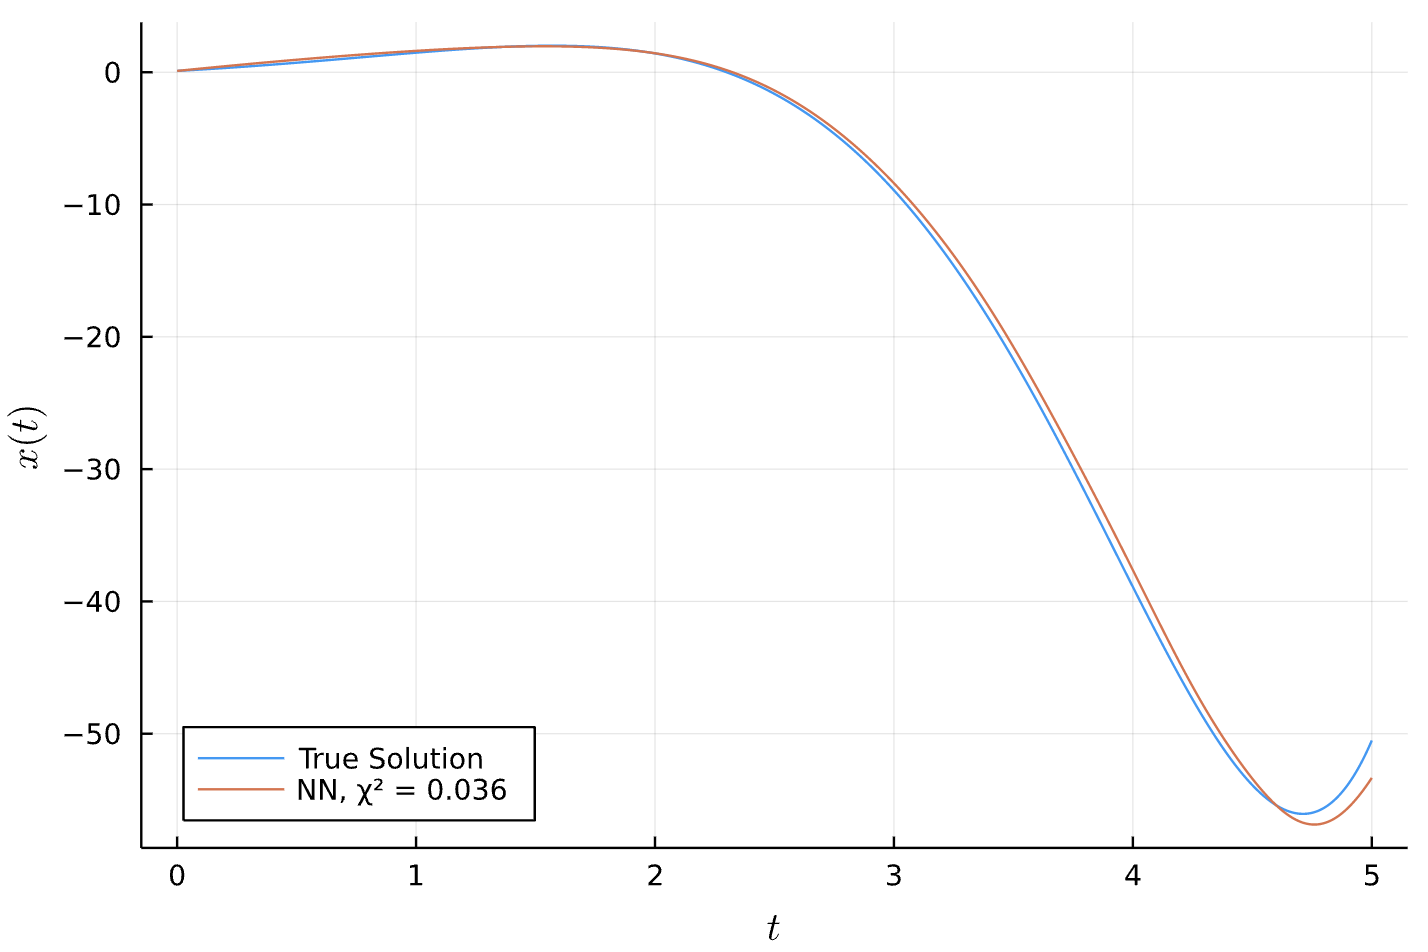
\includegraphics[width=0.45\linewidth]{figures/ODE_example.png}
\end{center}
and we see that our network does pretty well! We could, of course, improve performance by training longer or playing with the size of the network or learning rate, however the above remains a good example of how to utilize neural networks to solve ODEs as is. 

%% ---------------------------------------------------------------
%% SOLVING PDES WITH PINN
%% ---------------------------------------------------------------

\section{Solving PDEs with Physics-Informed Neural Networks}

We now turn our attention to solving partial different equations using techniques from scientific machine learning. We will use the package \texttt{NeuralPDE.jl} \cite{zubovNeuralPDEAutomatingPhysicsInformed2021} to solve some examples. 

Consider a partial differential equation given by 

\begin{equation}
	f(u(x); \lambda) = 0
\end{equation}
where $x \in \Omega$ are the independent variables in the space $\Omega$, $u(x)$ is the solution, $f$ is some non-linear function acting on $u$, and $\lambda$ are the parameters of the equation. To solve with a neural network $\net(x, w)$ where $\net$ is a neural network with weights $w$, we want to fulfill 

\begin{equation}
	f(\net(x, w); \lambda) \approx 0.
	\label{eqn:NNapprox}
\end{equation}
The universal approximation theorem tells us that this should be possible. The error of the above equation is then given by 

\begin{equation}
	\loss(w) = \int_{\Omega} ||f(\net(x,w); \lambda)||\,dx. 
	\label{eqn:NNloss}
\end{equation}
We have suggestively named the error $\loss$ as we can use this function as a loss function in training our neural network $\net$ by minimizing $\loss$. Our computational problem then reduces to the problem of evaluating the integral in Eqn. \ref{eqn:NNloss} in order to perform minimization. 

Notice that in practical problems, we apply boundary conditions $b_i$ on $\partial \Omega \in \Omega$ in order to obtain, ideally, a unique solution. In order to include this information in the network, we add in these conditions to our loss function giving us 

\begin{equation}
	\loss(w) = \sum_i\int_{\Omega\setminus\partial\Omega} ||f_i(\net(x,w); \lambda)||\,dx + \sum_i\int_{\partial\Omega} ||b_i(\net(x,w); \lambda)||\,dx.
	\label{eqn:complete_loss} 
\end{equation}
where we have generalized the problem to a system of coupled differential equations $f_i$. If we can find a way to efficiently evaluate this integral, then we can apply standard minimization algorithms to solve. 

\subsection{Methods of discretization}

There are several different methods for evaluating the integral in Eqn. \ref{eqn:complete_loss} namely: grid approximation techniques, stochastic grid approximation techniques, and machine learning (quadrature) techniques. A simple grid approximation takes the space $\Omega$ and divides it into units of volume $\Delta V$ with a specific length. The PDE is evaluated at each of this points and scaled by the volume, thus our integral is computed via 

\begin{equation}
	\int_{\Omega} ||f(\net(x,w); \lambda)||\,dx = \sum_i \Delta V ||f(x_i)||.
\end{equation}
This method has two main disadvantages: 1) as the dimension of the problem increases, the number of points we sample increases exponentially in order to maintain the same granularity and 2) no evaluation of the integral is done between grid points, thus information can be quickly lost. To solve the second problem, we can use stochastic methods of sampling---i.e., Monte Carlo techniques to evaluate the integral. This can be described by 

\begin{equation}
	\int_{\Omega} ||f(\net(x,w); \lambda)||\,dx = \alpha \sum_i ||f(x_i)||.
\end{equation}
for some scaler $\alpha$. As we simply want to minimize this integral, there is no need to specify $\alpha$. This problem still suffers from dimensionality exponentially increasing. Thus, we turn to a third method: quadrature training with a neural network. Several processes for specifying quadrature are described in \cite{riveraQuadratureRulesSolving2022}. These are typically of the form 

\begin{equation}
	\int_{\Omega} ||f(\net(x,w); \lambda)||\,dx = \sum_i \alpha_i ||f(x_i)||\,dx.
\end{equation}
In the implementation via \texttt{NeuralPDE.jl}, this is accomplised using the \texttt{Integrals.jl} package which calls the \Julia differential equation solver \cite{rackauckasDifferentialEquationsJlPerformant2017} to find the correct sampling points $x_i$ and weights $\alpha_i$ in an implementation of Gaussian quadrature rules. 

\subsection{Example using \texttt{NeuralPDE.jl}}

We show how \texttt{NeuralPDE.jl} can be used to solve a simple example and describe the important components of the code. 

Consider the homogeneous system of linear PDEs given by

\begin{equation}
\begin{split}
	\partial_t u - \partial_x v + (v + u) & = 0 \\
	\partial_t v - \partial_t u + (v + u) & = 0
\end{split}
\end{equation}
subject to the initial conditions 

\begin{equation}
	u(0,x) = \sinh x, \,\,\,\,\,\,\,\, v(0,x) = \cosh x. 
\end{equation}    
By means of the so-called Homotopy analysis method, the authors in \cite{samibatainehApproximateAnalyticalSolutions2008} find the analytical solution to this system to be given by 

\begin{equation}
	u(x,t) = \sinh(x - t), \,\,\,\,\,\,\,\, v(x,t) = \cosh(x - t). 
\end{equation}

We now solve with \texttt{NeuralPDE.jl}, describing important aspects of the code. To begin, we set up the system symbolically with the aid of \texttt{Modelingtoolkit.jl} as follows:

\begin{jllisting}
@parameters t x
@variables u(..) v(..)

Dx = Differential(x)
Dt = Differential(t)

eqns = [Dt(u(t,x)) - Dx(v(t,x)) + (u(t,x) + v(t,x)) ~ 0,
        Dt(v(t,x)) - Dx(u(t,x)) + (u(t,x) + v(t,x)) ~ 0]

bcs = [u(0,x) ~ sinh(x), v(0,x) ~ cosh(x)]

domains = [x ∈ Interval(0.0, 1.0),
            t ∈ Interval(0.0, 1.0)]

@named pde_sys = PDESystem(eqns, bcs, domains, [t,x], [u(t,x), v(t,x)])
\end{jllisting}
For systems of equations, store each equation as an element of the vector \texttt{eqn} as with the boundary conditions, \texttt{bcs}. We now define a neural network to solve the problem using the machine learning library \texttt{Lux.jl}. Our network has one hidden layer with 30 nodes, and takes two input variables---one for each parameter of the problem. We output a single number. Notice that each variable $u,v$ of our problem gets its own network. This is implemented simply as

\begin{jllisting}
dim = length(domains) # number of dimensions
n = 30
chains = [Lux.Chain(
            Dense(dim, n, Lux.σ), 
            Dense(n, n, Lux.σ), 
            Dense(n, 1)) for _ in 1:2]
\end{jllisting}
We then discretize the system using quadrature training as follows

\begin{jllisting}
strategy = QuadratureTraining()
discretization = PhysicsInformedNN(chains, strategy)
@time prob = discretize(pde_sys, discretization)
\end{jllisting}
After this is set-up and a loss function is defined through calling \texttt{PhysicsInformedNN}, we simply need to train the network to find a nice solution. This is done with the \texttt{Optimization.jl} library. We choose the ADAM optimizer over three learning rates: $10^{-3}, 10^{-4}$, and $10^{-7}$ over 10000, 7000, and 1000 epochs respectively. By training the network with successively smaller learning rates, we can improve the accuracy of the solution. This is accomplished in the following code:

\begin{jllisting}
i = 0
loss_history = []

callback = function (p,l) 
	global i += 1
	if i % 100 == 0
		println("Current loss is: $l")
	end
    append!(loss_history, l)
	return false 
end

learning_rates = [1e-3, 1e-4, 1e-7]
res = @time Optimization.solve(prob, ADAM(learning_rates[1]); callback = callback, maxiters=10000)
loss_history1 = loss_history
loss_history = []
prob = remake(prob, u0=res.minimizer)
res = @time Optimization.solve(prob, ADAM(learning_rates[2]); callback = callback, maxiters=7000)
loss_history2 = loss_history
loss_history = []
prob = remake(prob, u0=res.minimizer)
res = @time Optimization.solve(prob, ADAM(learning_rates[3]); callback = callback, maxiters=1000)
loss_history3 = loss_history
loss_history = vcat(loss_history1, loss_history2, loss_history3)
phi = discretization.phi
\end{jllisting}

The loss is displayed in Fig. \ref{fig:loss_linear} and the results of the above learning are shown in Fig. \ref{fig:results_linear}. Notice the instability of the loss at higher learning rates. Fixing these instabilities is accomplished with a lower learning rate as this requires that over each epoch movement in loss-space is limited. The results demonstrate that our learning was successful. 

\begin{figure}
\centering
	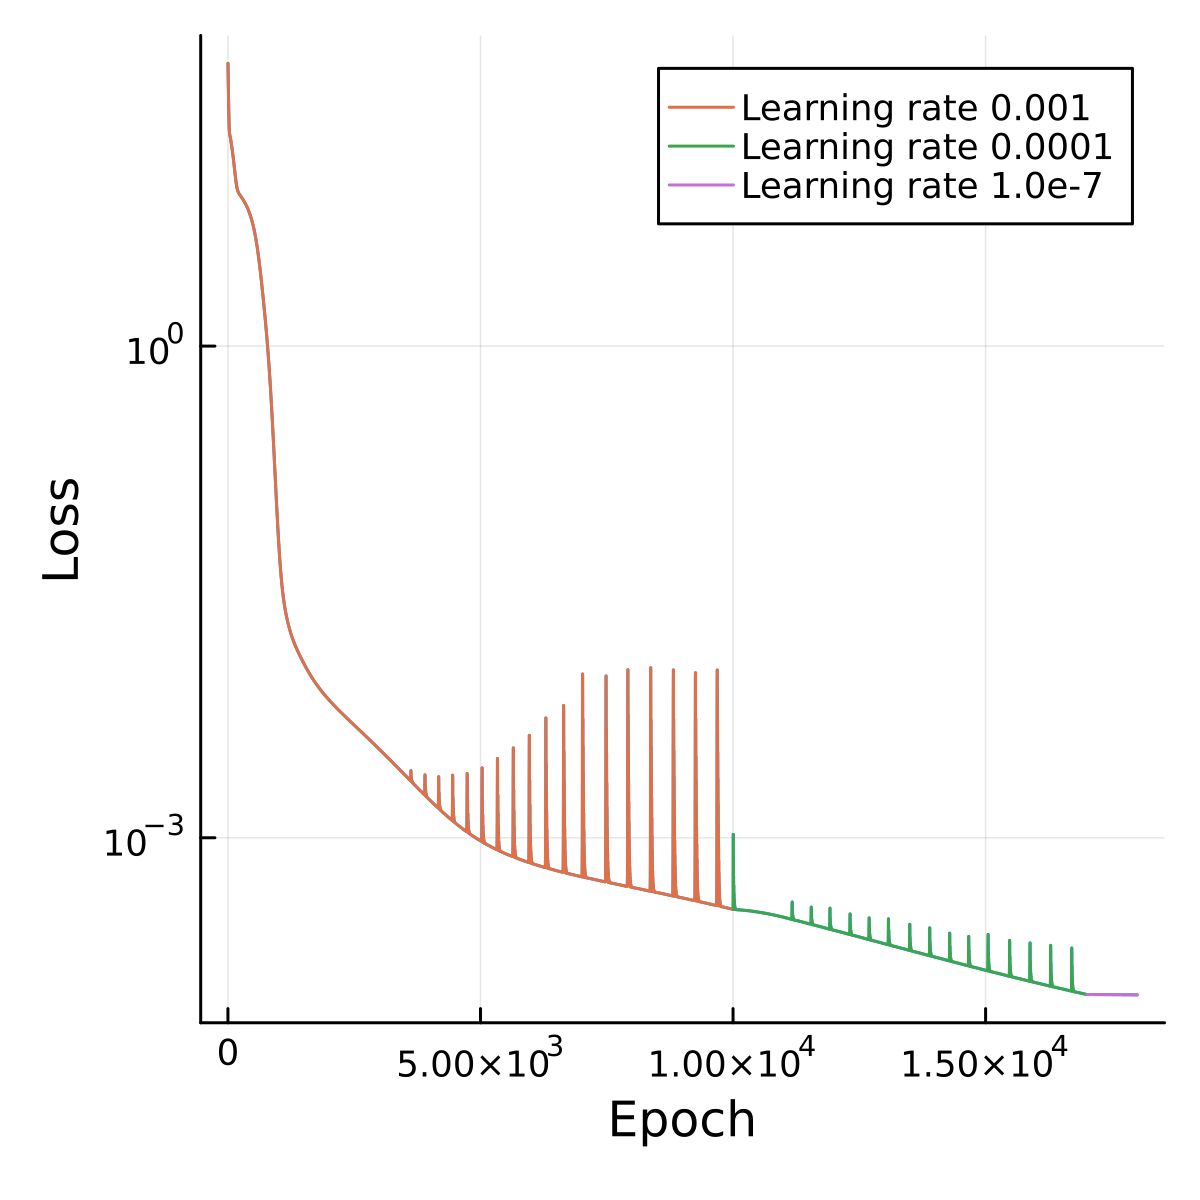
\includegraphics[width=0.4\linewidth]{figures/linear_homo_PDE_plots/loss.png}
	\caption{Value of loss as a function of epoch for the linear system of homogenous PDEs. Three stages of learning are represented with the learning rate labeled. While there are some instabilities in the loss, we ultimately find a nice solution with the final learning rate of $10^{-7}$}
	\label{fig:loss_linear}
\end{figure}

\begin{figure}
\centering
	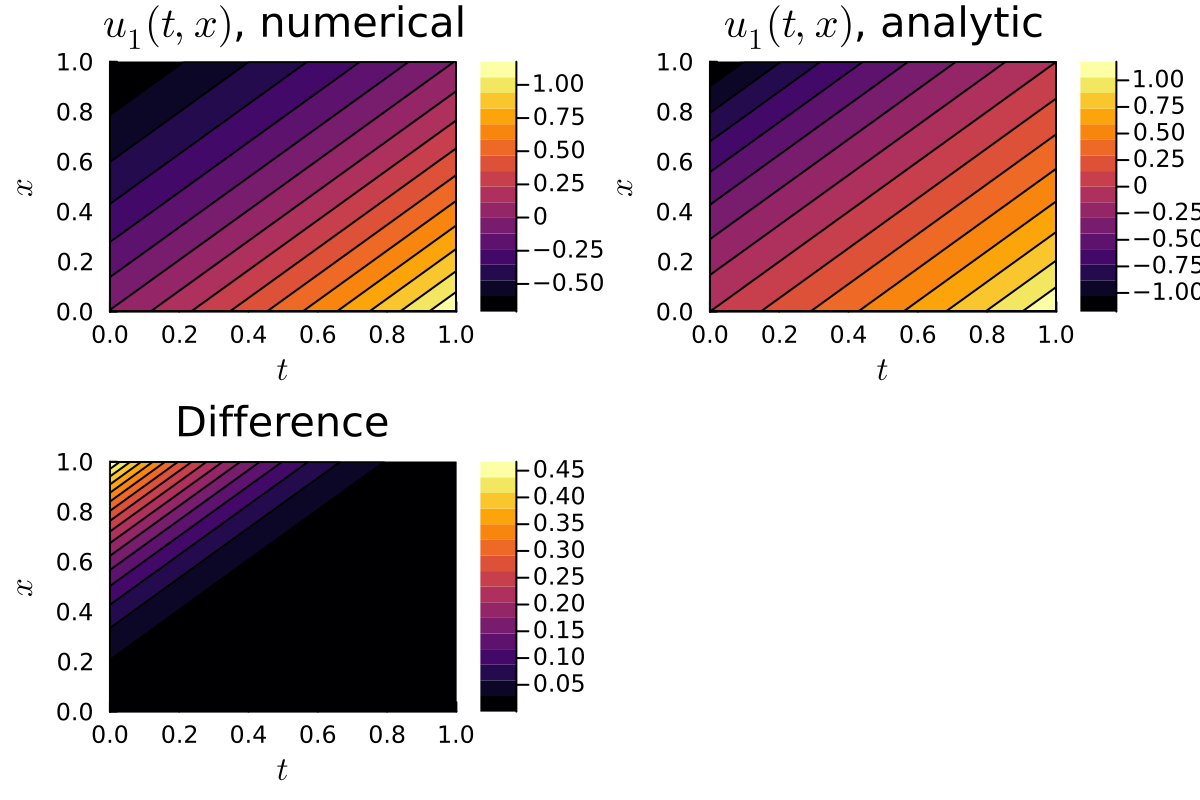
\includegraphics[width=0.48\linewidth]{figures/linear_homo_PDE_plots/solution_1.png}
	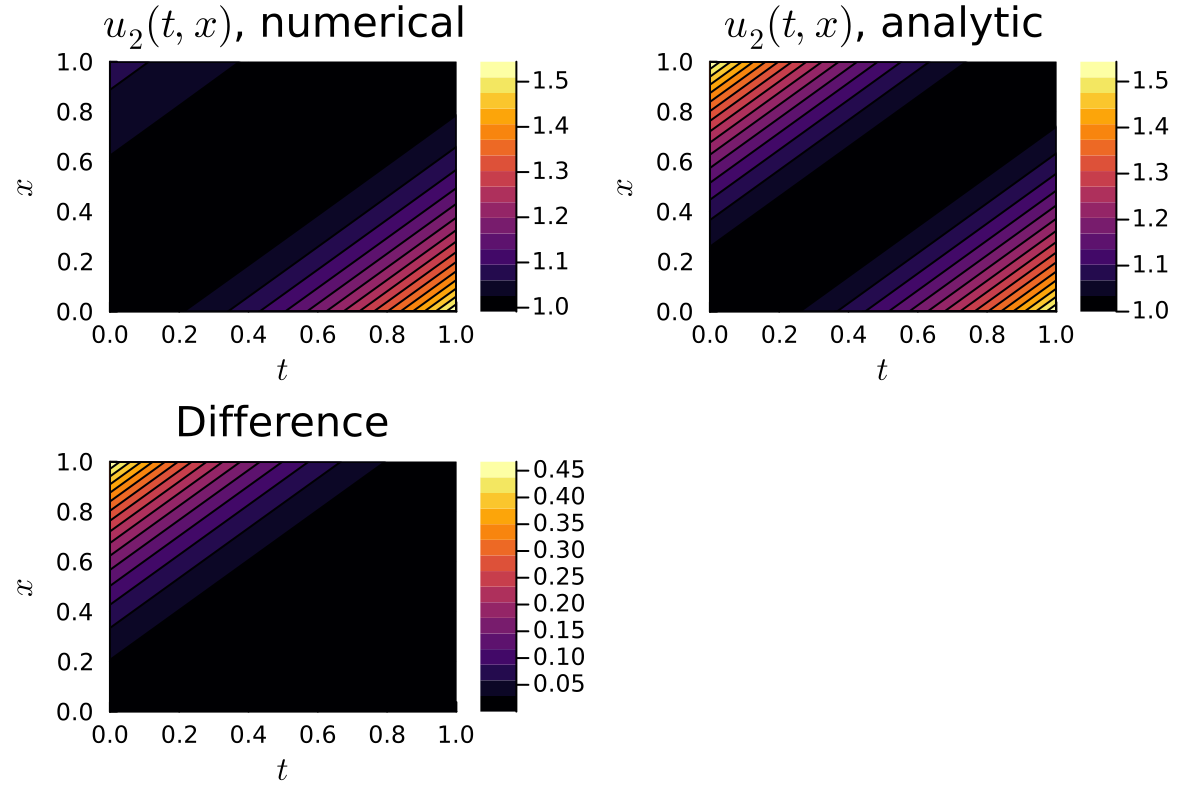
\includegraphics[width=0.48\linewidth]{figures/linear_homo_PDE_plots/solution_2.png}
	\caption{Results of training a neural network to learn the solution of the linear homogenous PDE. Solution $u$ is represented by $u_1$ and $v$ by $u_2$. In both cases, numerical and analytic solutions are shown as well as the difference between numerical and analytic defined by $|u_{numerical} - u_{analytic}|$}
	\label{fig:results_linear}
\end{figure}

\subsection{Solving Similarity Solution of Navier-Stokes using \texttt{NeuralPDE.jl}}

In the 1994 paper investigating the Blow-up of solutions to Navier-Stokes equations, Budd \textit{et al.} consider the system of PDEs arising from the Navier-Stokes equations under the geometry of an infinite channel \cite{buddBlowupSystemPartial1994}. In particular, they explore the parabolic partial differential equations perturbed from a similarity solution of the Navier-Stokes given by

\begin{equation}
\begin{split}
    \partial_t u_1 + \mu u_2 \partial_x u_1 & = \partial^2_{x} u_1 + u_1^2 - K^2, \,\,\,\,\,\,\,\, 0 < x < 1, 0 < t < T \\
    \partial_x u_2 & = u, \,\,\,\,\,\,\,\, 0 < x < 1, 0 < t < T
    \label{eqn:ns_problem}
\end{split}
\end{equation}
with the boundary conditions 

\begin{equation}
    \partial_x u_1(t,0) = \partial_x u_1(t,1) = u_2(t,0) = u_2(t,1) = 0
\end{equation}
and initial condition 

\begin{equation}
    u_1(x,0) = u_0(x).  
\end{equation}
These equations are parameterized by $\mu$, which perturbs the equations from Navier-Stokes. It is the goal of the paper to determine for which values of $\mu$ the solutions ``blow up." We will consider exclusively the case where $\mu = 1$, as this has a nice solution and the resulting system arises from the Navier Stokes equations as discussed below:

\subsubsection{Problem Derivation}

We consider the incompressible Navier-Stokes equations in an infinitely long channel in the $x$- and $z$-direction and finite in the $y$ direction; namely we bound $y$ by $0 < y < 1$. Let $u_1, u_2, u_3$ be velocity fields, $1/\nu$ be the Reynolds number, and $p$ be the pressure. Then, the Navier-Stokes equations read

\begin{equation}
    \begin{split}
        \partial_t u_1 - u_1^2 + u_2\partial_yu_1 & = \nu \partial_y^2 u_1 - c(t) \\
        \partial_t u_2 + u_2 \partial_y u_2 & = \nu \partial_y^2 u_2 - \partial_y p \\
        \partial_t u_3 - u_3^2 + u_2\partial_y u_3 & = \nu \partial_y^2 u_3 - e(t) \\
        \partial_y u_2 & = u_1 + u_3. 
    \end{split}
\end{equation}
In order to simplify, let $u_3(y,t) = 0$, $e(t) = 0$ and $\nu = 1$ so that our system becomes 

\begin{equation}
    \begin{split}
        \partial_t u_1 - u_1^2 + u_2\partial_yu_1 & = \nu \partial_y^2 u_1 - c(t) \\
        \partial_t u_2 + u_2 \partial_y u_2 & = \nu \partial_y^2 u_2 - \partial_y p \\
        \partial_y u_2 & = u_1. 
    \end{split}
\label{eqn:partial_system}
\end{equation}
Now note that $p(t)$ can be determined once we know $u_1, u_2$ from the above first and last equation as the middle equation of Eqn. \ref{eqn:partial_system} is only dependent on $u_2$. Hence, we write our system as 

\begin{equation}
    \begin{split}
        \partial_t u_1 + u_2\partial_yu_1 & = \partial_y^2 u_1 + u_1^2 - c(t) \\
        \partial_y u_2 & = u_1. 
    \end{split}
\end{equation}
which matches Eqn. \ref{eqn:ns_problem} when $\mu = 1$ and under the condition that $y \rightarrow x$. In order to have a complete solution, we need only finding appropriate inital conditions. The condition $u_2(0,t) = u_2(1,t)$ follows naturally to disallow flow through the walls of the channel. In \cite{buddBlowupSystemPartial1994}, they also employ the boundary condition $\partial_y u_1 = 0$ to obtain the above complete initial conditions. Finally, we require $c(t) \ge 0$ so that we can write $c(t) = K^2$. 

\subsubsection{Solution with PINN and comparison to analytical solution}

Let's now solve this system! Notice that via integration by parts of the first equation in \ref{eqn:ns_problem} we get

\begin{equation}
    K^2 = 2\int_0^1 u_1^2 \, dx. 
\end{equation}
Thus, we solve the system

\begin{equation}
    \begin{split}
        \partial_t u_1 & = \partial_x^2 u_1 - u_2 \partial_x u_1 + u_1^2 - 2\int_0^1 u_1^2 \,dx \\
        0 & = \partial_x u_2 - u_1
    \end{split}
\end{equation}
for $0 < x < 1$ and $0 < t < 1$. Using the same initial conditions as above, we set $u_0(x) = \cos \pi x$, coinciding with the analytical solution given in \cite{benhammoudaAnalyticalSolutionsSystems2014}. Using power-series methods, the authors find the analytical solution to the above system to be

\begin{equation}
    \begin{split}
        u_1(t,x) & = e^{-\pi^2t}\cos \pi x \\
        u_2(t,x) & = \frac{1}{\pi}e^{-\pi^2t} \sin \pi x. 
    \end{split}
\end{equation}

We can then solve the problem using \texttt{NeuralPDE.jl}. This differs from the above code only in the definition of an integral through \texttt{Modelingtoolkit.jl} which can simply be done with

\begin{jllisting}
Ix = Integral(x in DomainSets.ClosedInterval(0, 1))
\end{jllisting}

In this example we use the sigmoid as our activation function and build a network with one hidden layer of fifteen nodes. The input layer of our network must be the length of the number of parameters defined in our problem. Additionally, we use a different neural network for each solution $u_1$ and $u_2$ of our system, thus we define two neural networks with the set-up described above. The discretization we choose is the quasi random training with 100 points (ADD MORE DESCRIPTION!!). 

For optimization we use the ADAM optimizer and vary the learning rate starting with a rate of 0.1 over 500 epochs, then 0.01 over 2000 epochs, then finally $10^{-4}$ over a final 2000 epochs. The loss over these epochs and learning rates can be seen in Fig. \ref{fig:loss_integro} and the solution can be seen in Fig. \ref{fig:integro_results}.

\begin{figure}
\centering
    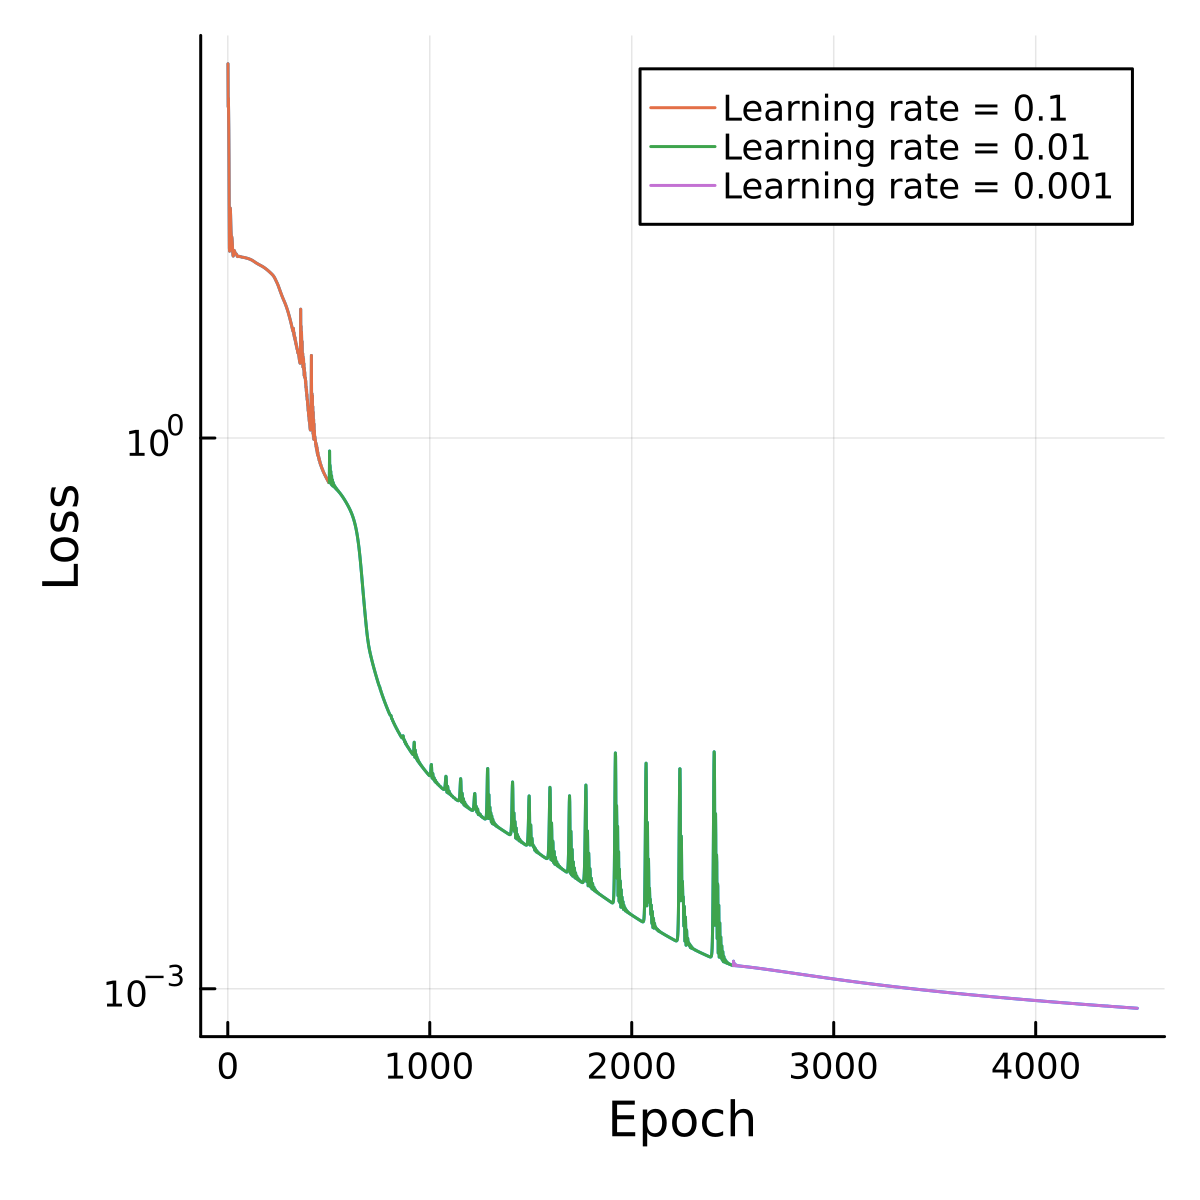
\includegraphics[width=0.4\linewidth]{figures/integral_PDE_plots/loss.png}
    \caption{Loss as a function of epoch in training a neural network to learn the solution of the integral PDE presented above. Learning is broken up into three sections with differing learning rate as shown}
    \label{fig:loss_integro}
\end{figure}

\begin{figure}
\centering
    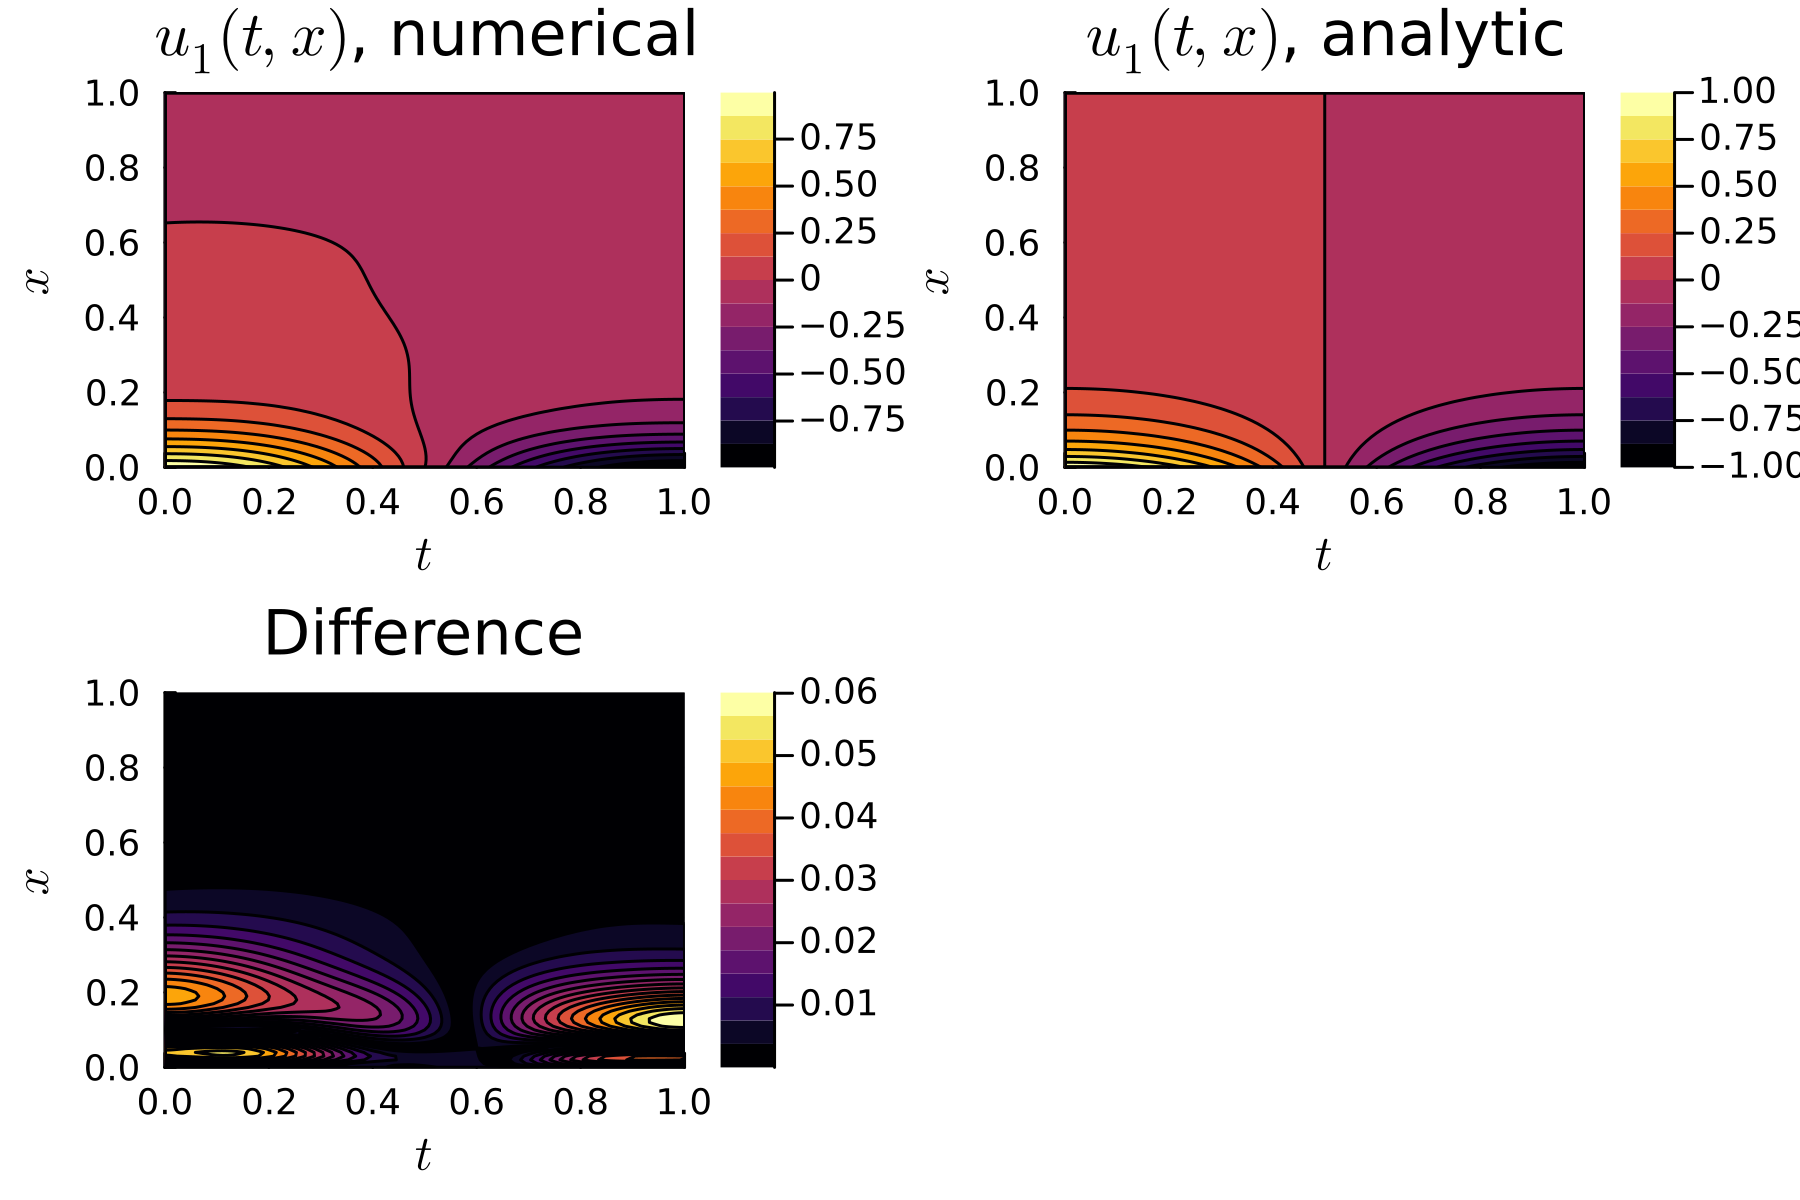
\includegraphics[width=0.48\linewidth]{figures/integral_PDE_plots/plot_u1.png}
    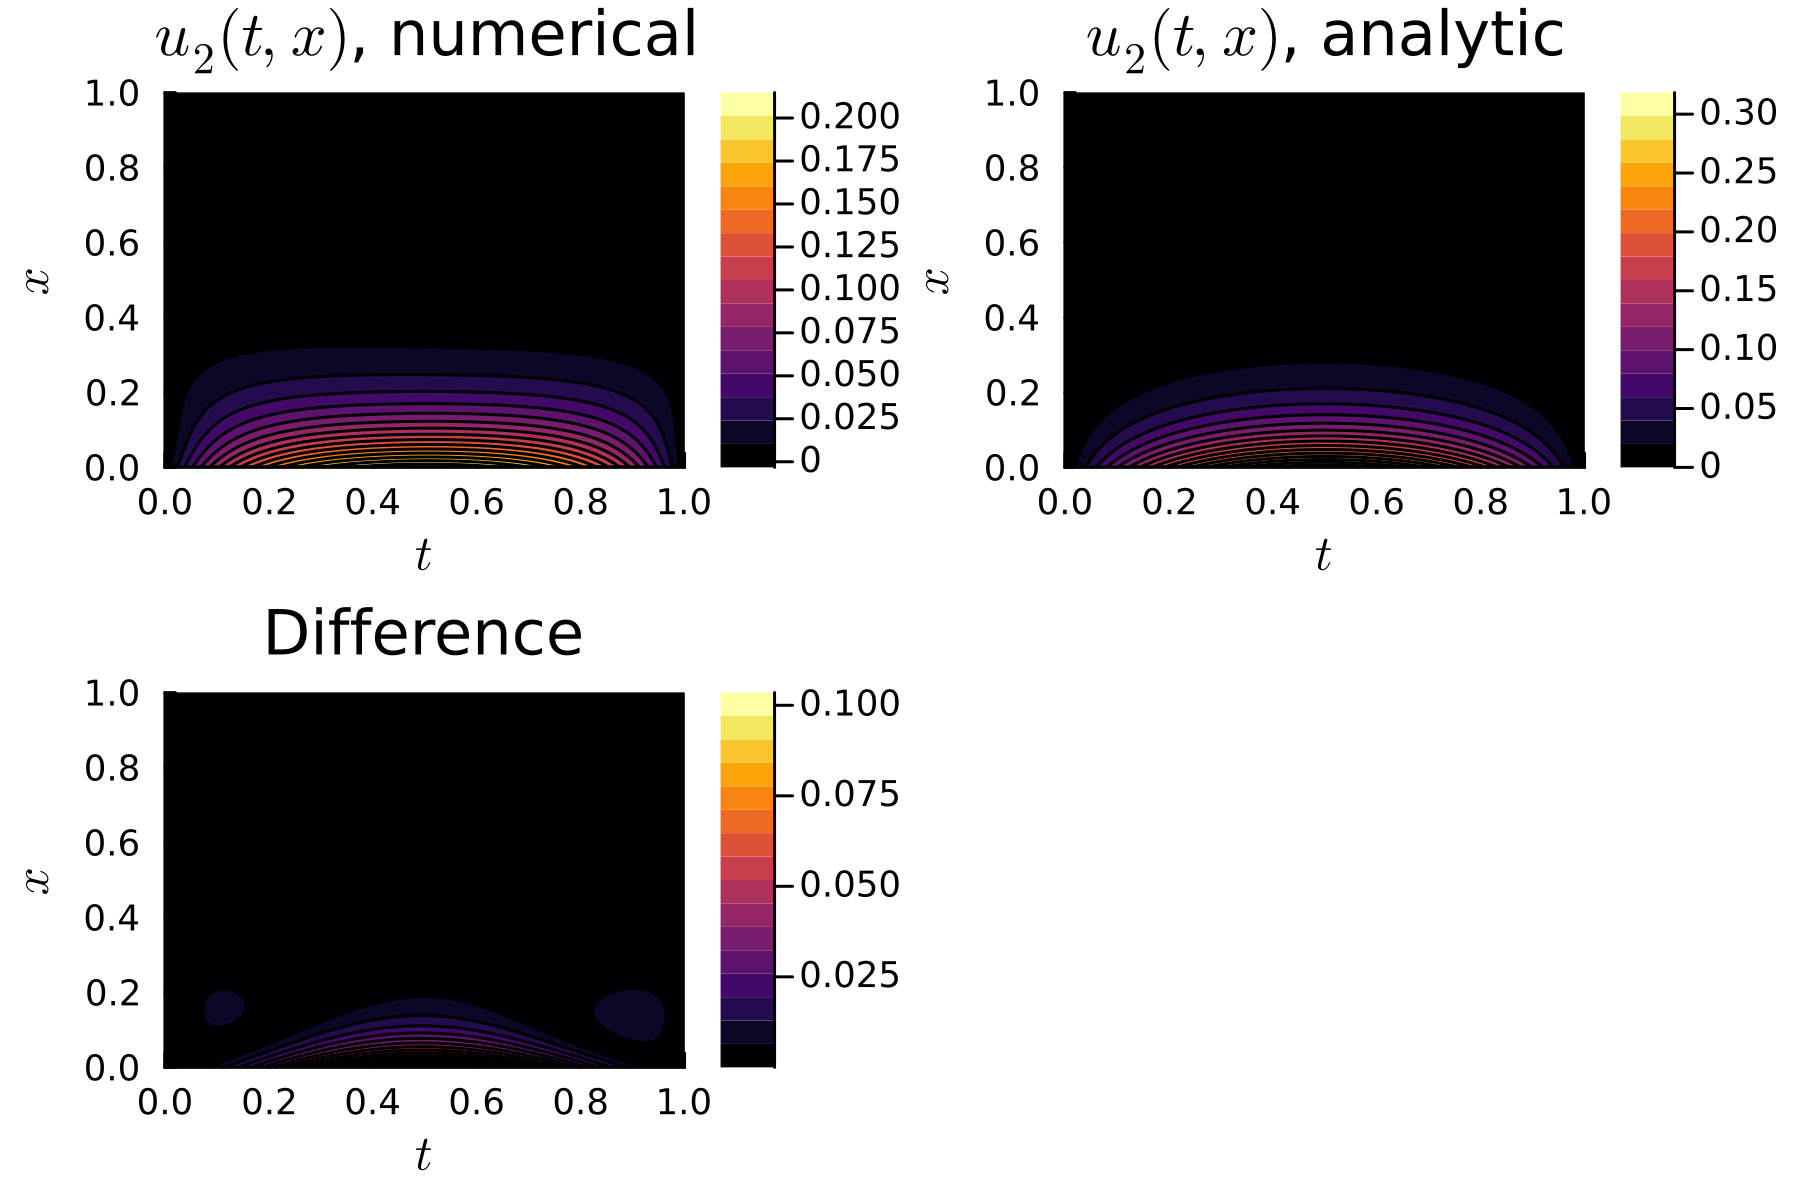
\includegraphics[width=0.48\linewidth]{figures/integral_PDE_plots/plot_u2.png}
    \caption{Results of training a network to learn the solution of the integral PDE. Both numerical and analytical solutions are given with the difference between the two. We see that the numerical solution matches the analytic solution very well.}
    \label{fig:integro_results}
\end{figure}

To see the complete implementation of the above, see the data availability statement. 

%% ---------------------------------------------------------------
%% SECTION: SOLVING EFE
%% ---------------------------------------------------------------

\section{Solving Einstein's Field Equations to obtain the Schwarzschild Metric using \texttt{NeuralPDE.jl}}

We find a numerical solution to Einstein's field equations resulting in the Schwarzschild Metric as first described by Schwarzschild in 1916 \cite{schwarzschildGravitationalFieldMass1999} by using PINN techniques and mathematical simplifications. This problem has the benefit that it both tests the limits of what neural networks can do while still having a nice analytical solution. 

\subsection{Physics Background and Problem Set-up}

Solutions to the Einstein field equations seek to describe space-time, mathematically encapsulated in the space-time metric tensor $g_{\mu\nu}$. We will consider the problem of a massive black hole which is 1) uncharged and 2) non-rotating following the detailed solution given in \cite{eigenchrisRelativity108aSchwarzschild}. To find $g_{\mu\nu}$, consider Einstein's field equations given by 

\begin{equation}
    R_{\mu\nu} - \frac{1}{2}R g_{\mu\nu} + \Lambda g_{\mu\nu} = \frac{8 \pi G}{c^4}T_{\mu\nu}.
    \label{eqn:EFE}
\end{equation}
We will consider space-time outside the black hole which we assume to be empty. Thus, $T_{\mu\nu} = 0$. We additionally will not consider cosmological scales so we just set $\Lambda = 0$. Using some algebra, we then find that

\begin{equation}
\begin{split}
    R_{\mu\nu} - \frac{1}{2}Rg_{\mu\nu} & = 0 \\
    R_{\mu\nu}g^{\mu\nu} - \frac{1}{2}Rg_{mu\nu}g^{\mu\nu} & = 0 \\
    R - 2R & = 0 \\ 
    R_{\mu\nu} & = 0 \implies \boxed{R_{\mu\nu} = 0}. 
\end{split}
\end{equation}
Define the Cristoffel symbols as

\begin{equation}
    \Gamma^{\alpha}_{\mu\nu} := -\frac{1}{2}\sum_{\beta}g^{\alpha\beta}\left(\frac{\partial g_{\mu\beta}}{\partial x_{\nu}} + \frac{\partial g_{\nu\beta}}{\partial x_{\mu}} - \frac{\partial g_{\mu\nu}}{\partial x_{\beta}}\right).
    \label{eqn:ccs}
\end{equation}
Subsequently, we define the Ricci tensor as:

\begin{equation}
    R_{\mu\nu} := \sum_{\alpha} \frac{\partial \Gamma^{\alpha}_{\mu\nu}}{\partial x_{\alpha}} - \sum_{\alpha} \frac{\partial \Gamma^{\alpha}_{\alpha\mu}}{\partial x_{\nu}} + \sum_{\alpha\beta} \left(\Gamma^{\alpha}_{\alpha\beta} \Gamma^{\beta}_{\mu\nu} - \Gamma^{\alpha}_{\mu\beta} \Gamma^{\beta}_{\alpha\nu}\right)
    \label{eqn:ricci}
\end{equation}
Finally, define the metric tensor as 

\begin{equation}
    g_{\mu\nu} = \begin{pmatrix}
        g_{00} & g_{01} & g_{02} & g_{03} \\
        g_{10} & g_{11} & g_{12} & g_{13} \\
        g_{20} & g_{21} & g_{22} & g_{23} \\
        g_{30} & g_{31} & g_{32} & g_{33}
    \end{pmatrix}
\end{equation}
where we use the space-time indices $(0,1,2,3)$ corresponding to the variables $(ct, \rho, \theta, \phi)$ in spherical coordinates. 

In order to solve we need to make a few further assumptions:

\begin{enumerate}
    \item As $r \rightarrow \infty$, $g_{\mu\nu} \rightarrow \eta_{\mu\nu}$ where $\eta_{\mu\nu}$ is the minkowski metric in sphereical coordinates. 
    \item Space-time is static meaning that a) $\partial_t g_{\mu\nu} = 0$ and b) $t \rightarrow -t$ leaves $g_{\mu\nu}$ unchanged. This ensures the black hole is non-rotating. 
    \item Space-time is spherically symmetric. 
\end{enumerate}
Applying these assumptions to the metric yields 

\begin{equation}
    g_{\mu\nu} = \begin{pmatrix}
        A(r) & 0 & 0 & 0 \\
        0 & -B(r) & 0 & 0 \\
        0 & 0 & r^2 & 0 \\
        0 & 0 & 0 & r^2\sin^2\theta
    \end{pmatrix}.
    \label{eqn:g_simple}
\end{equation}
Finally, in order to find a unique solution, we need to ensure the metric matches Newtonian gravity in the limits of 1) weak gravity and 2) low velocity. This essentially means we need the Geodesic Equation, given by 

\begin{equation}
    \frac{d^2 x^{\sigma}}{d\lambda^2} + \Gamma^{\sigma}_{\mu\nu} \frac{dx^{\mu}}{d\lambda}\frac{dx^{\nu}}{d\lambda} = 0,
    \label{eqn:geo}
\end{equation}
to match Newtonian gravity, given by 

\begin{equation}
    \frac{d^2x^i}{dt^2} + \frac{\partial\varphi}{\partial x^i} = 0
    \label{eqn:newton}
\end{equation}
where $\varphi = -GM/r$ is the gravitational potential. 

\begin{enumerate}
\item In the limit of low velocity, $t \approx \tau = ct$, and a particle's four-velocity is dominated by the time component so that $\textbf{U} = (c,0,0,0)$. This reduces Eqn. \ref{eqn:geo} to 

\begin{equation}
     \frac{d^2x^i}{dt^2} + \Gamma^i_{00}c^2 = 0
     \label{eqn:geo_low_v}
\end{equation}
which implies that 

\begin{equation}
    \Gamma^i_{00} = \frac{\partial \varphi}{\partial x^i}\frac{1}{c^2}. 
\end{equation}

\item In the limit of weak gravity we write $g_{\mu\nu} \approx \eta_{\mu\nu} + h_{\mu\nu}$ where $||h_{\mu\nu}|| \ll 1$. Then, we can write 

\begin{equation}
    \Gamma^i_{00} = \frac{1}{2}\eta^{ii}(\partial_0 h_{i0} + \partial_0h_{i0} - \partial_i h_{00})
\end{equation}
as derivatives of the constant matrix $\eta$ in Cartesian coordinates are zero. Because all off-diagonal elements of our matrix are zero, this reduces to 

\begin{equation}
    \Gamma^i_{00} = -\frac{1}{2}\eta^{ii}\partial_i h_{00}
\end{equation}
where we note that $\eta^{ii} = -1$ in Cartesian coordinates. 
\end{enumerate}

Applying all the above conditions, we find that the metric is given by

\begin{equation}
    g_{\mu\nu} = \begin{pmatrix}
        1 - \frac{r_s}{r} & 0 & 0 & 0 \\
        0 & -(1 - \frac{r_s}{r})^{-1} & 0 & 0 \\
        0 & 0 & r^2 & 0 \\
        0 & 0 & 0 & r^2\sin^2\theta
    \end{pmatrix},
\end{equation}
where 

\begin{equation}
    r_s = \frac{2GM}{c^2}
\end{equation}
is the Schwarzschild radius or the event horizon of the black hole. 

\subsection{Technical Implementation}

While this system has a nice, simple analytical solution, finding a numerical solution is not trivial. In particular, starting with Eqn. \ref{eqn:ricci} and then applying the assumptions outlined above as initial conditions yields a PDE problem too big to feasibly solve given the time constrains of this capstone. For this reason, we will use the simplified form of $g_{\mu\nu}$ given in Eqn. \ref{eqn:g_simple} for our implementation. While this yields a system of highly coupled ODEs, employing initial conditions such that a solutions is reached is still not trivial. The implementation provided also demonstrates how the problem may be expanded to more dimensions at the cost of significantly longer training times as we use \texttt{NeuralPDE.jl} to solve. Additionally, architecture for expanding to more complex systems is included in the implementation for potential future use. 

The system of equations we ultimately solve can be found by plugging the form of Eqn. \ref{eqn:g_simple} into Eqn. \ref{eqn:ricci}. This results in the system given by 

\begin{equation}
\begin{split}
    4A'B^2 - 2rB''AB + 2A'B'B + rB'^2A & = 0 \\
    rA'B + 2A^2B - 2AB - rB'A & = 0 \\ 
    -2rB''AB + rA'B'B + rB'^2A - 4B'AB & = 0
    \label{eqn:einstein_ODEs}
\end{split}
\end{equation}
where the prime indicates a derivative of $r$ such that $A' = dA(r)/dr$. In order to fulfill the condition $r \rightarrow \infty$, $g_{\mu\nu} \rightarrow \eta_{\mu\nu}$, we impose the boundary conditions $A(r_{max}) = 1, B(r_{max}) = 1$. We solve this problem over the interval $r = [r_{min}, r_{max}]$ where we choose $r_{min}$ such that $r_{min} > r_s$ to avoid the singularity at the black-hole's event horizon, and $r_{max}$ is big enough such the boundary condition is a reasonable approximation when applied to the analytic solution. Recall that the analytical solution is given by 

\begin{equation}
\begin{split}
    A(r) & = 1 - \frac{r_s}{r} \\ 
    B(r) & = -\left(1 - \frac{r_s}{r}\right)^{-1}
\end{split}
\end{equation}
where $r_s$ is the Schwarzschild radius. 

For this problem, we will consider space-time around a black hole with a weight $10^5$ times that of the sun and will use astronomical units for length and years for time. Thus, $GM = 3.94\si{AU^{3}/year^2}$ and $c = 6.3 \times 10^4 \si{AU/year}$ so that $r_s = 1.2 \times 10^{-4} \si{AU}$. 

Our problem in almost completely defined, however, we still need to find a way to match Newtonian gravity in the limit of low velocity and weak gravity. In order to do this, we put a test particle into the space-time predicted by our network and let this particle move according to Eqn. \ref{eqn:geo_low_v}. We then drop this same particle into a Newtonian space-time and let it move according to Eqn. \ref{eqn:newton}. We can then compare the predictions of both and add this prediction to the loss function for training a solution. This is done simply by using the euclidean distance metric and squaring such that the closer the two points are to each other in space, the smaller the loss is. 

Unfortunately, implementing this is not a trivial task. Notice that in order for the network to learn or perform backpropogation, the ODE given in Eqn. \ref{eqn:geo_low_v} must must be solved \emph{inside the loss function}. Moreover, in order to move towards a better solution, we must be able to take the derivative of an ODE solver: a clear application of differentiable programming. Moreover, solutions to the simple Newtonian version can quickly blow-up or require advanced solving techniques for slight changes in initial parameters of the problem. This makes solving within the loss function potentially very unstable. 

In order to partially overcome an unstable loss, we pick a solution to the Newtonian problem which slowly moves away from a stable orbit. In addition, we solve only in the $x-y$ plane so as to eliminate as much computational pressure as possible. By placing our particle on the $x$-axis with velocity completely in the $y$-direction, namely we place it at $(40 \si{AU}, 0 \si{AU})$ with velocity $(0 \si{AU/yr}, 500 \si{AU/yr})$ we accomplish these conditions. Solving over the time interval $t = (0, 0.1)$ with \texttt{DifferentialEquations.jl} yields the solution shown in Fig. \ref{fig:newton_sol}. 

Now that we have the system setup, we can attempt to solve the problem in Eqn. \ref{eqn:einstein_ODEs}. We use a network with two hidden layers both with the sigmoid activation function. Each hidden layer contains ten nodes each. Weights in the network are initialized uniformly according to the Glorot paper \cite{glorotUnderstandingDifficultyTraining2010}. Training is done with the BFGS and limited memory BFGS algorithm \cite{liuLimitedMemoryBFGS1989} over fifteen epochs. 

\begin{figure}
    \centering
    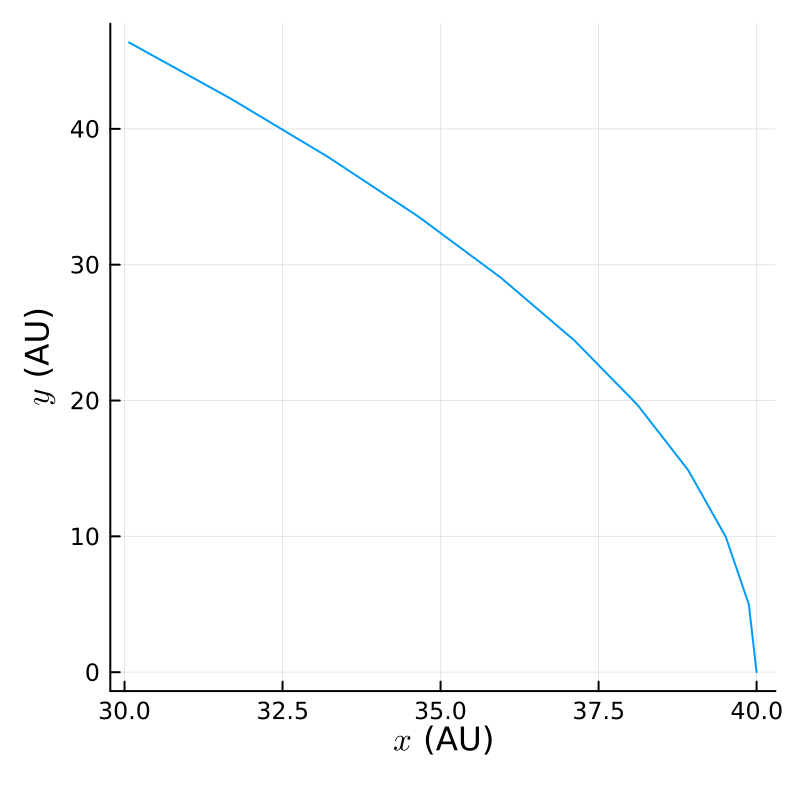
\includegraphics[width=0.3\linewidth]{figures/newton_solution.png}
    \caption{Caption}
    \label{fig:newton_sol}
\end{figure}

\subsection{Results and Discussion}

%% ---------------------------------------------------------------
%% SECTION: CONCLUSION
%% ---------------------------------------------------------------

\section{Conclusion}

%% ---------------------------------------------------------------
%% BACKBATTER, MISC. 
%% ---------------------------------------------------------------

\begin{Backmatter}

\paragraph{Acknowledgments}

I am very grateful for the mentorship of Alex Heaton and Megan Pickett in working on this project. Additionally, none of this would have been possible without the education I have received at Lawrence University. I would like to thank the Physics and Mathematics department for their support and all of the opportunities I have had through both departments. 

\paragraph{Data Availability Statement} All code presented above can be found in my Github, \hyperlink{https://github.com/lvb5/solve\_PDEs\_with\_PINN}{github.com/lvb5}. 

\bibliography{references}
\bibliographystyle{ieeetr}

\end{Backmatter}

\end{document}

% The solutions outlined in Swarzschild's paper yields the following differential equations to solve

% \begin{equation}
%     \sum_{\alpha} \frac{\partial \Gamma^{\alpha}_{\mu\nu}}{\partial x_{\alpha}} + \sum_{\alpha\beta} \Gamma^{\alpha}_{\mu\beta} \Gamma^{\beta}_{\mu\alpha} = 0
% \end{equation}
% where we also require 

% \begin{equation}
%     |g_{\mu\nu}| = -1. 
% \end{equation}

% %% EXTRA EXAMPLE

% \begin{example}

% Consider the PDAE given by 

% \begin{equation}
%     \begin{split}
%         \partial_t^2 u_1 & = \partial_x^2 u_1 + u_3 \sin \pi x \\
%         \partial_t^2 & = \partial_x^2 + u_3 \cos \pi x \\
%         0 & = u_1 \sin \pi x + u_2 \cos \pi x - e^{-t}
%     \end{split}
% \end{equation}
% on the intervals $0 < x < 1$, $t > 0$. We require the initial conditions

% \begin{equation}
%     \begin{split}
%         u_1(0,x) & = \sin \pi x \\
%         \partial_t u_1(0,x) & = -\sin \pi x \\
%         u_2(0,x) & = -\sin \pi x \\
%         \partial_t u_2(0,x) & = -\cos \pi x
%     \end{split}
% \end{equation}
% and the boundary conditions

% \begin{equation}
%     \begin{split}
%         u_1(t,0) & = u_1(t,1) = 0 \\
%         u_2(t,0) & = -u_2(t,1) = e^{-t}. 
%     \end{split}
% \end{equation}
% The exact solution to this system is given by 

% \begin{equation}
%     \begin{split}
%         u_1(t,x) & = e^{-t}\sin \pi x \\
%         u_2(t,x) & = e^{-t}\cos \pi x \\
%         u_3(t,x) & = (1+\pi^2)e^{-t}
%     \end{split}
% \end{equation}
% for $0 \le x \le 1$, $t \ge 0$. 

% \end{example}
